\chapter{Models for symbol grounding in games}
% TODO: title

\label{ch:fluents}

% TODO: name Symbol grounding in games
% TODO: par about grounding?

In Chapter~\ref{ch:rl}, we've presented how to apply Deep Reinforcement
Learning to achieve non-Markovian goals. We've seen that a construction based
on temporal logics, that we call the Restraining Bolt, is an elegant solution
that transforms the original problem to a classic MDP, by producing additional
rewards and observations. We report the general scheme here, in
Figure~\ref{fig:rb-focus-features}.
\begin{figure}
	\centering
	\begin{tikzpicture}[
			every node/.append style={font=\small},
			arrow/.style={->, semithick},
		]
		\matrix [
			 row sep=0.5cm, column sep=1cm,
		] {
			\node (env) [block, minimum size=2cm] {World}; \& \& \&
			\node (agent) [block, minimum size=2cm] {Learning\\agent}; \\
			\&
			\node (features) [block, fill=lightgray] {Features\\extractor}; \&
			\node (rb) [block] {Restraining\\Bolt}; \& \\
		};
		\coordinate (a1) at ($(agent.west)+(0,0.5)$);
		\draw [arrow] (a1) -- node [near start, above] {$a$} (env.east |- a1);
		\coordinate (w1) at ($(env.east)+(0,-0.2)$);
		\draw [arrow] (w1) -- node [near start, above] {$r$} (agent.west |- w1);
		\coordinate (w2) at ($(env.east)+(0,-0.5)$);
		\draw [arrow] (w2) -- node [near start, below] {$o$} (agent.west |- w2);
		\draw [arrow] (w2) ++(0.5,0) |- (features.west);
		\draw [arrow] (features) -- node [near start, above] {$l$} (rb);
		\draw [arrow] ($(rb.east)+(0,0.1)$) -- ++(0.3,0)
			|- node [below right] {$\vec{q}$} ($(agent.west)+(0,-0.8)$);
		\draw [arrow, dashed] ($(rb.east)+(0,-0.1)$)
			-| node [near end,right] {$r'$} (agent.south);
	\end{tikzpicture}
	\caption{In this chapter, we focus on the features extractor.}
	\label{fig:rb-focus-features}
\end{figure}
The two blocks at the bottom are our additions, and part of the solution.
We've thoroughly addressed the Restraining Bolt in Section~\ref{sec:rb},
already. In this chapter, we want to focus on the other essential component:
the features extractor.

The purpose of the features extractor is to receive an observation from the
environment and produce a Boolean valuation for some predefined propositional
symbols, that we call fluents. We assume that the set of fluents~$\fluents$
has already been defined, and the truth of every atomic proposition
in~$\fluents$ can be decided from a single input~$o$. This means that if we
did define a symbol that cannot be decided from one observation, for example a
generic ``$\const{GoalReached}$'' condition, we need to split that symbol into
much simpler events, and define $\const{GoalReached}$ in terms of the new
fluents.

Usually, the features extractor is not a really interesting component. Once,
we've defined a fluent~$\fluent \in \fluents$, we could manually program a
function, $f_\fluent: \obsS \to \B$, that predicts when that event occurs or
that condition is verified\footnote{$\B$ is the set $\set{0, 1}$, which
represents $\set{\false, \true}$.}.  This approach is perfectly fine, when
applicable.  However, the environments used in Deep Reinforcement Learning
usually produce high-dimensional or noisy observations. As we may imagine, it
becomes really hard to manually classify such inputs in the two classes. So,
in order to apply the Restraining Bolt or any other logic-based method to Deep
RL, we must resort to some Machine Learning model that will help us deciding
the truth of our atomic propositions.

Any Deep RL agent processes the input observation with a Neural Network. A
reasonable choice would be to use a NN also as model for the features
extractor. We may use a joint network that predicts the value for every fluent
defined: $f: \obsS \to \B^{\abs{\fluents}}$. The simplest way to train this
model is through supervised learning, where we provide many input-output
samples. Supervised learning can generate very accurate models, but, for every
image in the training dataset, we would need to manually label the desired
outputs, i.e. the fluents that are true in that image. Unfortunately, the
effort of this manual intervention would completely dominate over the
advantages of the high-level, logic approach. If possible, we would certainly
like to avoid this manual work. 

A very promising alternative is unsupervised learning. These models don't
return predictions. Instead, they memorize patterns and features that the
training inputs have in common. These models keep two representations: the
input space, and the latent space. To any input that is presented to the
model corresponds a compact representation in the latent space. The purpose
of this representation is to distinguish the specific input among all of the
training set\footnote{To emphasize this concept: the latent vector serves to
identify the input sample among the training distribution.}. Since the latent
vector is much more compact, it can be used in other computations in place of
the original input. In this case, the latent vector is called an
\emph{encoding}.

Unsupervised learning will be a central part of the solution proposed here.
However, it may not be the only part, because unsupervised models makes no
guarantees about the meaning of the latent representation. This means that
we cannot predict what each number in the latent vector represents. So, the
proposed model will transform the encodings through a second function, which
computes the truth value of the fluents.

To better understand the motivation behind our choices, we list few general
goals that we want to pursue with this work:
\begin{enumerate}
	\item Learning should not require manual labelling.
	\item \label{en:select-fluents} We select the fluents that should be learnt.
	\item \label{en:generic-model} Model should make as few environment-specific
		assumptions as possible.
\end{enumerate}
The second principle means that we first choose the propositions to use in our
temporal formulae, then we train a model to valuate them. An opposite approach
could have been to train an extractor of Boolean features, then trying to
recognize the meaning of those fluents.

With the general goals~\ref{en:select-fluents} and~\ref{en:generic-model}
above, in particular, we express that the model should be generalizable to a
wide range of output fluents and input observations. Of course, this is only
possible to some extent. As we'll discuss in
Section~\ref{sec:fluents-assumptions} and~\ref{sec:fluents-limitations}, this
method, as realized in this thesis, makes some assumptions that limit its
applicability to a specific class of fluents and observations. However, this
work poses some interesting ideas, such as temporal constraints, that
certainly needs to be further investigated in the future. This thesis is just
an initial study in this direction.


\section{Temporal constraints}

In this section, we illustrate the concept of ``temporal constraints''. This
is an important idea introduced with this work, that will help us pursue the
three principles above. We can start from the following observation: a dataset
of labelled samples is a description, by examples, of the desired meaning of
the fluents. A good model would interpolate between these samples to inputs
that have never been observed. Without these examples, how do we specify the
desired meaning of a fluent? Note that by ``meaning'', we mean the set of
inputs in which the propositional symbol should be valuated to true.

What we propose here is to specify the desired temporal behaviour of these
fluents with temporal logics: we write a temporal formula, in \ltl{} or
\ldl{}, that describes all the possible traces of the fluents we want to
define. We don't talk about \emph{desired} trajectories. Instead, we define
all the \emph{possible} trajectories according to the environment dynamics.
For example, suppose that two conditions $A$ and $B$, according to their
intended meaning, cannot be true at the same time. Regardless of what we're
trying to achieve, we can write the following temporal constraint:
$\lbox{\true^*}(\lnot A \lor \lnot B)$.  This is a simple propositional
property that should hold in every instant, but there are many other
interesting constraints that we may specify with temporal logic. For example,
$A$ and $\ldiamond{\true^*}(\llast \land A)$ respectively mean: every episode
starts/ends with an instant where $A$ is true.  Also, $\lbox{\true^*;
A}\ldiamond{\true^*}B$ means that every time $A$ becomes true, the event $B$
must follow later on. This is a frequent pattern in request--response
behaviours. The automaton associated to this constraint is shown in
Figure~\ref{fig:response-automa}.
\begin{figure}
		\centering
		\begin{tikzpicture}
		\graph [
			automaton, grow right=3cm,
		]{
			0 [accept] -> ["$A$"] 1;
			0 -> [self loop above, "$\lnot A$"] 0;
			1 -> [self loop above, "$A \lor \lnot B$"] 1;
			1 -> [backward, "$B \land \lnot A$"] 0;
		}; 
		\draw [init path] (0.west) +(-0.5,0) -- (0.west);
		\end{tikzpicture} 
		\caption{The DFA associated to the formula ${\lbox{\true^*;
			A}\ldiamond{\true^*}B}$.}
		\label{fig:response-automa}
\end{figure}
% TODO: note about symbolic transitions?
Temporal logics like \ldl{} are very expressive and allows to write many
complex properties that the symbols satisfy.

Usually, we won't be able to write complete constraints or exact definitions
of the fluents. This is not necessary, though. It is sufficient to exclude as
many inconsistent trajectories as we can, given the symbols available.

\begin{example}
	Suppose that an agent should open a door that is closed with a key, and
	we've defined the fluents $\fluents \coloneqq \set{\const{HaveKey},
	\const{DoorOpen}}$. We need to train a feature extractor that valuates these
	two propositions with their intended interpretation. We may write the
	following constraint:
	\[
		(\lnot \const{HaveKey} \land \lnot \const{DoorOpen})
		\land \lnot \ldiamond{\true^*; \lnot \const{HaveKey}}\const{DoorOpen}
	\]
	which says that the door cannot be opened if, at the previous instant, we
	don't have a key. Also, initially, the door is closed and the agent has no
	key.  The associated automaton is shown in Figure~\ref{fig:door-automa}.
	\begin{figure}[tb]
			\centering
			\begin{tikzpicture}
			\graph [
				tree layout, automaton, level distance=2cm, sibling distance=3cm,
			]{
				0 [accept] -> {
					1 [accept, >"$\lnot\const{DoorOpen} \land \lnot\const{HaveKey}$"]
						-> ["$\const{HaveKey} \land \lnot\const{DoorOpen}$", bend right]
						2 [accept],
					3 [>"$\const{DoorOpen} \lor \const{HaveKey}$"']
				},
				3 -> [clear >, "$\true$", self loop right] 3,
				1 -> [clear >, "$\const{DoorOpen}$"] 3,
				2 -> [clear >, "$\lnot\const{HaveKey}$", bend right] 1,
				2 -> [clear >, "$\const{HaveKey}$", self loop below] 2,
				1 -> ["$\lnot\const{DoorOpen} \land \lnot\const{HaveKey}$",
					self loop left] 1
			}; 
			\draw [init path] (0.north) +(0,0.5) -- (0.north);
			\end{tikzpicture} 
			\caption{The DFA associated to the Example~\ref{ex:door}.}
			\label{fig:door-automa}
	\end{figure}
	Note that we didn't specify that the door should be eventually opened. The
	automaton only excludes the trajectories that certainly can't happen.
	\label{ex:door}
\end{example}

The general idea is shown in Figure~\ref{fig:constraints-scheme}. We're
trying to learn the unknown function $f: \obsS \to \B^{\abs{\fluents}}$,
which, from a single input observation, computes the truth value for all
fluents. The trace generated must always satisfy the temporal constraint
defined in~$\constraintS$.
\begin{figure}[bt]
	\centering
	\begin{tikzpicture}[
			every pin/.style={font=\footnotesize},
			node distance=0.7cm,
		]
		% Inputs
		\node (frame0) [image, xshift=-0.4cm, yshift=0.4cm, opacity=0.5]
			{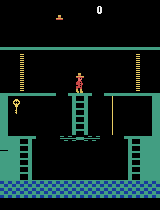
\includegraphics[width=1cm]{./imgs/mz0.png}};
		\node (frame1) [image, xshift=-0.2cm, yshift=0.2cm, opacity=0.8]
			{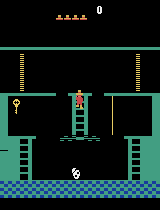
\includegraphics[width=1cm]{./imgs/mz1.png}};
		\node (frame2) [image]
			{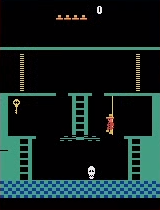
\includegraphics[width=1cm]{./imgs/mz3.png}};
		\node (frames) [fit=(frame0) (frame2), pin=above:{input sequence}] {};
		% Function
		\draw [->, thin, draw=lightgray] (frame0.east) ++(0.7,0) -- ++(2,0)
			coordinate (fn0-right);
		\draw [->, thin, draw=gray] (frame1.east) ++(0.7,0) -- ++(2,0)
			coordinate (fn1-right);
		\path (frame2.east) ++(0.7,0) edge [arrow]
			node [midway, auto=right, outer sep=0.7ex,
					pin={[pin edge=pin line]below:{unknown\\valuation function}}] {
				$f: \obsS \to \B^{\abs{\fluents}}$}
			coordinate [at end] (fn2-right) ++(2,0);
		% Output
		\begin{scope}[every matrix/.style={
			matrix of nodes, nodes in empty cells,
			row sep=-\pgflinewidth, column sep=-\pgflinewidth,
			nodes={anchor=center, draw, minimum width=1.1em, minimum height=1.1em,
				font=\footnotesize, inner sep=3pt, fill=white},
			cells={draw},
		}]
			\matrix (values0) [right=of fn0-right, nodes={draw=lightgray, thin}] {
				\\\\\\\\\\
			};
			\matrix (values1) [right=of fn1-right, nodes={draw=gray, thin}] {
				\\\\\\\\\\
			};
			\matrix (values2) [right=of fn2-right] {
				1\\1\\0\\1\\0\\
			};
		\end{scope}
		\node (values) [fit=(values0) (values2), pin={output trace}] {};
		% Constraint
		\draw (values2.east) ++(0.5,0) edge [thick, dashed]
			node [midway, auto=right, outer sep=0.7ex,
					pin=below:{temporal constraint}]
				{$\trace \models \constraintS$}
			coordinate [at end] (line-right) ++(2,0);
		\node (formula) [right=0.5cm of line-right] [pin=above:{\ldl{} formula}]
			{\constraintS};
	\end{tikzpicture}
	\caption{The trace generated by the valuation function must satisfy the
	temporal constraint.}
	\label{fig:constraints-scheme}
\end{figure}

We've just described how temporal constraints work. However, there is one
important consideration to do: these constraints are very weak. This means
that there will be lots of fluents' valuations functions that are consistent
with this specification. Consider Example~\ref{ex:door}, a feature
extractor~${f(o) \coloneqq \set{}}$ completely ignores the input and always
predicts that both fluents are false. It is wrong but it's perfectly
consistent with the specification. Similarly, many other valuation functions
that respect the DFA dynamics of Figure~\ref{fig:door-automa} will be
completely meaningless.  This may not surprise us, as most constraints can
only relate the valuation functions with each other, but they cannot force
arbitrary input--output associations. The initial and final conditions (such
as $\lnot \const{HaveKey} \land \lnot \const{DoorOpen}$ in the
Example~\ref{ex:door}) are some of the few examples that creates a strong
binding between input observations and desired fluents' output.


\section{Assumptions}

\label{sec:fluents-assumptions}

In this section, we'll list the initial choices and assumptions taken in this
work.  Of course, assumptions like these restrict the range of valuation
functions that can be learnt. However, they are essential in order to devise a
solution.  The purpose of most of them is to address the issue mentioned in
the previous section: temporal constraints are only very weak indications of
the desired meaning of the fluents. Other assumptions, instead, describe the
range of environments which the proposed model can be applied to.

First, we remember that the environments we're dealing with are video games
from the Atari collection.  So, the input space is composed of images of size
$(210, 160)$. In the following, we will always use images from this games,
because this is how environment's observations look like.

Then, we assume that each atomic proposition can be decided just from a fixed
region of the input image. In other words, to each fluent, we associate a
rectangular portion of the input and we assume that an observation of this
region is sufficient to decide the truth of the symbol. Regions can overlap
and different fluents can be defined on the same region. By restricting the
input space of the model so much, we're partially reducing the complexity of
the problem.  

\begin{example}
	In order to better understand what regions are, we anticipate one
	environment that we'll encounter in the experiments
	Section~\ref{sec:exp-breakout}: Breakout. In this famous game, the player's
	goal is to direct the ball toward the bricks. Suppose we want to learn three
	fluents~$\fluents \coloneqq \set{\const{Empty}, \const{Full},
	\const{PaddleLeft}}$, as shown in Figure~\ref{fig:assumption-ex-breakout}.
	\begin{figure}
		\centering
		\begin{tikzpicture}[
				every node/.append={font=\footnotesize},
				small arrow/.style={->, thin, >=spaced stealth'},
			]
			\node [image, outer sep=0pt] (env-br)
				{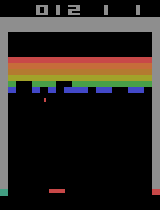
\includegraphics[height=3cm]{./imgs/br2.png}}; \&
			\begin{scope}[
					shift=(env-br.north west), x={(env-br.north east)},
					y={(env-br.south west)}]
				\draw [region box] \boxblueright node (blueright) {};
				\draw [region box] \boxpaddleleft node (paddleleft) {};
			\end{scope}
			\matrix (bluem) [matrix of math nodes, right=of blueright] {
				\const{Full} \\ \const{Empty} \\
			};
			\node (leftn) [left=of paddleleft] {$\const{PaddleLeft}$};
			\draw [small arrow] (bluem-1-1) -- (blueright-|env-br.east);
			\draw [small arrow] (bluem-2-1) -- (blueright-|env-br.east);
			\draw [small arrow] (leftn) -- (paddleleft-|env-br.west);
		\end{tikzpicture}
		\caption{Fluents and regions for the environment Breakout in
		Example~\ref{ex:assumption-ex-breakout}.}
		\label{fig:assumption-ex-breakout}
	\end{figure}
	The region associated to each of these symbols is indicated with an orange
	box. $\const{PaddleLeft}$ should be true when the paddle is inside the
	area on the left; $\const{Empty}$ and $\const{Full}$ should be true
	respectively when all the bricks, or no bricks, inside the region have been
	shot down.
	\label{ex:assumption-ex-breakout}
\end{example}

As it may be clear from this example, the regions also help to do something
that would be impossible in logic: indicate to which portion of the input the
fluents refer. Also, we should choose each region as a small selection of
the image in which the condition we'd like to extract is \emph{visually
evident}: to different valuations should correspond noticeable differences
in the region. In the following sections, we'll refine what we mean by
``noticeable''. Essentially, we mean that the model must be able to learn an
encoding that captures the properties we're interested in. Unfortunately,
this is not something that can be described with extreme precision, in machine
learning. We'll discuss this issue in Section~\ref{sec:encoding-what-learns}.

Due to these fixed regions, this method is only applicable to games with a
fixed view of the scene. If every object in the image were moving, we
couldn't apply the simplification of static regions. Few examples of games
that respect this constraint are: Breakout, Mr.~Pac-Man, Video Pinball, Pong.
We'll also experiment with Montezuma's Revenge, but we'll limit to the first
room.

In Section~\ref{sec:fluents-limitations},
``\nameref{sec:fluents-limitations}'', we'll suggest few ideas about how many
of these limitations might be relaxed.


\section{General structure of the model}

\label{sec:model-structure}

In this section, we introduce the general structure of the model that we
propose in this thesis. The remaining parts of the chapter will cover all the
details and definitions.

As we already know, temporal constraints can exclude many inconsistent
assignments but they are only weak indications about the desired valuation
functions. By assuming regions, we've strongly reduced the size of the input
space, hence of the possible functions. Still, the problem is only mitigated.
To address this issue, we propose to learn each valuation function from an
encoding vector that represents the region of interest, rather than from the
pixel values directly. An encoding is a low-dimensional vector that represents
a more complex input. So, we might use this vector in place of the original
input in order to simplify the learning process of the valuation function.

An encoding can be viewed as a lossy compression of the input. The meaning of
the encoding vector depends on the specific model, which will be presented in
Section~\ref{sec:encoding}. Here, we only want to highlight that all input
images that are considered similar according to the model will correspond to
the same encoding vector. Hence, these images will produce the same
interpretation for the fluents. However, this is certainly a desirable effect:
the encoder can extract few relevant indicators from which we can compute the
fluents' values, while noises and tiny variations of the input will be
ignored.

So, the model that we propose is a function composed of two consecutive parts:
an array of \emph{encoders} and an array of \emph{Boolean functions}.  This
scheme is illustrated in Figure~\ref{fig:model-scheme}.
\begin{figure}
	\centering
	\begin{tikzpicture}[
			node distance=0.7cm,
			every label/.style={font=\scriptsize},
		]

		% Input
		\node [image] (frame)
			{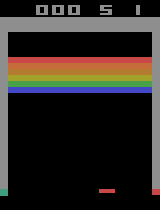
\includegraphics[height=2cm]{./imgs/br0.png}};
		\node [dot, right=0.7cm of frame] (input) {};

		% Encoders
		\matrix [
			right=of input, nodes={anchor=center},
			row sep=0.5cm, column sep=0.5cm,
		] (encoders) {
			\node [block] (encoder1) {Encoder\\(region 1)}; \&
			\node [dot] (encoded1) {}; \\
			\node [block] (encoder2) {Encoder\\(region 2)}; \&
			\node [dot] (encoded2) {}; \\
		};

		% Boolean functions & output
		\matrix [
			right=of encoders, nodes={anchor=center},
			row sep=0.3cm, column sep=1cm, label distance=0.4cm,
		] (boolfns) {
			\node [block] (boolfn1) {Boolean fn 1}; \&
			\node [label=right:Fluent 1] (output1) {0}; \\
			\node [block] (boolfn2) {Boolean fn 2}; \&
			\node [label=right:Fluent 2] (output2) {1}; \\
			\node [block] (boolfn3) {Boolean fn 3}; \&
			\node [label=right:Fluent 3] (output3) {0}; \\
		};

		% Output
		\node [draw, rectangle, gray, inner sep=0pt, fit=(output1) (output3)
			] (outputs) {};

		% Flow
		\draw (frame) to (input);
		\draw [->] (input) edge (encoder1) edge (encoder2);
		\draw (encoder1) to (encoded1);
		\draw (encoder2) to (encoded2);
		\draw [->] (encoded1) edge (boolfn1.west) edge (boolfn2.west);
		\draw [->] (encoded2) edge (boolfn3.west);
		\draw [->] (boolfn1) to (output1);
		\draw [->] (boolfn2) to (output2);
		\draw [->] (boolfn3) to (output3);

		% Models
		\begin{pgfonlayer}{below}
			\node (model) [
				fit=(input) (encoders) (boolfn1) (boolfn3),
				draw=blue!30!gray, fill=blue!40!gray!20!white,
				inner sep=0.2cm, label=above:{\normalsize Model},
			] {};
		\end{pgfonlayer}

		% Annotations
		\coordinate (annotations y) at ($(model.south)+(0,-0.8)$);
		\begin{pgfonlayer}{below}
			\node (input-annotation) at (input|-annotations y) {Input};
			\node (encoding-annotation) at (encoded1|-annotations y) {Encodings};
			\node (outputs-annotation) at (outputs|-annotations y) {Predictions};
			\draw [pin line] (input) -- (input-annotation);
			\draw [pin line] (encoded1) -- (encoding-annotation);
			\draw [pin line] (outputs) -- (outputs-annotation);
		\end{pgfonlayer}
	\end{tikzpicture}
	\caption{The model is composed by a sequence of encoders and a set of
	Boolean functions.}
	\label{fig:model-scheme}
\end{figure}
Let's assume that the set~$\fluents$ of fluents to learn is given, along with
their associated regions. We create an encoder for each region and a Boolean
function for each symbol in~$\fluents$. There might be less encoders than
Boolean functions, because multiple fluents can share the same region.
This scheme has two encoders and three Boolean functions (just like the model
associated to the example in Figure~\ref{fig:assumption-ex-breakout}). Of
course, that is just a specific instance. There will be as many parts as are
needed.

To summarize:
\begin{enumerate}
	\item The input frame is cropped around each region;
	\item Each small image is transformed with its own encoder;
	\item Each Boolean function computes the value for one fluent from the
		corresponding encoding vector.
\end{enumerate}


\section{Encoding}

\label{sec:encoding}

The encoder is a Machine Learning model that is trained in an unsupervised
way, whose purpose is to convert the input of one region to the associated
low-dimensional representation. The model we've selected for this role is the
Deep Belief Network. As we will see, this choice is mainly motivated by the
output produced by this model, which is a vector of binary features. In the
following, we'll thoroughly describe this model, and discuss why a binary
output is so important.

Since the layers of a Deep Belief Network are a specific type of Markov Random
Field, it is better to quickly review these first. This will allow us to
better understand the goal and properties of the final encoder.


\subsection{Markov Random Fields}

In the previous chapters, we have sometimes used Directed Graphical Models
(for example in Figure~\vref{fig:mdp}). These are probabilistic models in
which directed arcs represent known conditional probabilities between two
variables. Here, instead, we'll adopt a different kind of formalism:
\emph{Undirected Graphical Models} (UGMs)\nomenclature{UGM}{Undirected
Graphical Models}, which are also called \emph{Markov Random Fields}
(MRFs)\nomenclature{MRF}{Markov Random Fields}. Most of the topics presented
in this section are a reorganization of the material
in~\cite{bib:ml-book-murphy}.

A UGM is an undirected graph, where variables are represented by nodes, as
usual, and undirected arcs connect variables which are directly dependent.
A missing edge means that two variables are conditionally independent given
the others. For example, in Figure~\ref{fig:mrf}, $x_1$ and $x_4$ are
dependent variables, but they become conditionally independent if $x_2$ is
observed.
\begin{figure}
	\centering
	\begin{tikzpicture}
		\graph [
			spring layout,
			empty nodes, nodes=node,
			horizontal=x2 to x4,
		] {
			x1 [label=left:$x_1$] -- x2 [label=above:$x_2$] -- 
				x3 [label=left:$x_3$] -- x1,
			x2 -- x4 [label=right:$x_4$]
		};
	\end{tikzpicture}
	\caption{A small MRF where: $x_1 \not\perp x_4$, but $x_1 \perp x_4 \given
	x_2$.}
	\label{fig:mrf}
\end{figure}
In this and the following graphs, we assume that each node represents a scalar
quantity. Vectorial quantities will be indicated in bold fonts.

MRFs are very convenient when we what to express that two variables are
related, but we can't establish any causal relation between them. Consider,
for example, the noisy pixels of an image. The values of neighbouring pixels
are clearly dependent, as they are related by the subject of the image, but we
can't establish any useful conditional probability between the two.

In every MRF, the joint probability of all the variables can be expressed
as\footnote{In this chapter, vectors are denoted with bold lower-case letters.
So, the entries of a vector~$\x$ are~$x_i$. Similarly, matrices are indicated
with bold upper-case letters. A matrix~$\bvec{A}$ has columns~$\bvec{a}_{:j}$
and entries~$a_{ij}$.}:
\begin{equation}
	p(\x \given \params) \propto
		\prod_{c \in \setSym{C}} \psi_c(\x_c; \params_c)
\end{equation}
where each $c \in \setSym{C}$ is a maximal clique of the graph, and each
function $\psi_c$ computes how likely is the observation of variables~$\x_c$,
according to the parameters~$\params_c$. The joint probability is only
proportional to that quantity, because one normalizer has been omitted. As an
example, the joint probability for Figure~\ref{fig:mrf} can be written:
\[
	p(\x \given \params) \propto
	\psi_1(x_1, x_2, x_3; \params_1) \, \psi_2(x_2, x_4; \params_2)
\]

Therefore, a model for a MRF is fully defined by two factors: the structure of
the graph, and the functions~$\psi_c$. While the former strongly depends on
the process to be modelled, we can present the most common choice for the
latter. First, let's rewrite each term as:
\begin{equation}
	\psi_c(\x_c; \params_c) \coloneqq \exp(-E(\x_c; \params_c))
	\label{eq:ugm-energy-based}
\end{equation}
for some function~$E$. $E$ is called the \emph{energy function}. Since it is
inversely correlated to the probability, it is high for unlikely
configurations of variables and low for very probable configurations
(according to the model parameters, of course). Due to this property, the
energy is sometimes a very useful indication of the final
probability\footnote{Computing the exact probability $p(\x \given \params)$,
as many other quantities, is intractable for generic UGMs, because often we
won't be able to compute the normalizer.}.  Usually, the energy function is of
the simplest kind, a linear combination: $E(\x_c; \params_c) \coloneqq
-\params_c^T \basisfun_c(\x_c)$, for some basis function~$\basisfun_c$. In the
following, we'll assume this form.

As we may recognize, in a MRF there is no output. We're not trying to learn an
input--output function. Training a model means to find the optimal parameters
$\optimal\params$ that maximize the probability of the input samples. The
trained model should represent the probability distribution of the input data,
as closely as possible. This is clearly different from supervised learning.

Let's denote with $\dataset$ a dataset of training samples, $\dataset
\coloneqq \set{\x\group{i}}$, and with $l(\params)$ the log-probability of the
dataset according to the model, $l(\params) \coloneqq \log p(\dataset \given
\params)$. The optimal parameters are those maximizing the likelihood
$l(\params)$. So, we may approach this solution by following the positive
gradient of the likelihood. The gradient of the likelihood, with respect to
each group $c$ of parameters, is~\footnote{ The function $\basisfun_c$ only
receives the values of the clique $c$.  In the following equation, we write
$\x$ instead of $\x_c$, to ease the notation.}:
\begin{equation}
	\frac{\partial l}{\partial \params_c} = \E_{\x' \sim \dataset}
	\bigl[\basisfun_c(\x') \bigr] - \E_{\x} \bigl[\basisfun_c(\x) \bigr]
	\label{eq:ugm-gradient}
\end{equation}
The two parts compute the expected value of same quantity according to a
different distribution of~$\x$. The positive term simply stands for the
average value of that quantity, computed from the samples in the training
dataset; while in the right-most term, we take an expectation on $\x$
according to the distribution induced by the model.

We'll end this quick review of MRFs, by discussing the role of latent
variables. As we already know from the comparison between MDPs and POMDPs,
probabilistic models that include some unobservable variables can be much more
expressive than the others. Such variables are referred to as \emph{latent}
variables, or simply \emph{hidden} variables. The latent variables of a model
can be a very effective explanation of the visible quantities. Just like
the states of a POMDP explain the visible observations, a latent variable
representing the subject of an image is a clear motivation for the observed
pixel values. Connecting the visible units directly would be very hard to do.
Latent units in a MRF do not define such causal relations, but the added
expressiveness is the same.

We partition the units of the model as $\x = (\bv, \bh)$, where $\bv$ and
$\bh$ denote the visible and hidden variables, respectively. A model with
latent variables can be trained very similarly to what we've seen above. The
only difference to equation~\eqref{eq:ugm-gradient} is that we need to always
take the expectation on $\bh$ according to the model, because they will never
be observed in the dataset:
\begin{equation}
	\frac{\partial l}{\partial \params_c} = \E_{\bv \sim \dataset,\bh}
	\bigl[\basisfun_c(\bv, \bh)\bigr] - \E_{\bv,\bh} \bigl[\basisfun_c(\bv,
	\bh)\bigr]
	\label{eq:ugm-po-gradient}
\end{equation}


\subsubsection*{Restricted Boltzmann Machine}

The specific model that we'll use is the \emph{Restricted Boltzmann Machine}
(RBM)\nomenclature{RBM}{Restricted Boltzmann Machine}. An RBM is a MRF
composed of a visible and a hidden layer. Its graph is shown in
Figure~\ref{fig:rbm}.
\begin{figure}
	\centering
	\begin{tikzpicture}[
		node distance=1.2cm and 1.2cm, anchor=center
	]

	\node [node, label=above:$h_1$] (h1) {};
	\node [node, label=above:$h_2$, right=of h1] (h2) {};
	\node [right=of h2] (dots1) {\dots};
	\node [node, label=above:$h_H$, right=of dots1] (hK) {};

	\node [observed node, label=below:$v_1$, below=of h1, xshift=-0.7cm] (v1) {};
	\node [observed node, label=below:$v_2$, right=of v1] (v2) {};
	\node [observed node, label=below:$v_3$, right=of v2] (v3) {};
	\node [right=of v3] (dots2) {\dots};
	\node [observed node, label=below:$v_V$, right=of dots2] (vR) {};

	\graph {{(h1), (h2), (hK)} --[complete bipartite] {(v1), (v2), (v3), (vR)}};
	\end{tikzpicture}
	\caption{The UGM of a Restricted Boltzmann Machine. Gray nodes are the
	visible units.}
	\label{fig:rbm}
\end{figure}
As we can see, there are no connections between variables of the same layer,
and every clique has two nodes. So, the joint probability is simply:
\begin{equation}
	p(\bv, \bh) \propto \prod_{i=1}^{V} \prod_{j=1}^{H} \psi_{ij}(v_i, h_j)
	\label{eq:rbm-joint-psi}
\end{equation}
with one function $\psi_{ij}$ for each arc $(v_i, h_j)$. This simplification,
along with other nice properties, are only possible thanks to its bipartite
structure. This is why it is said ``restricted''. Useful RBMs have strictly
less hidden than visible units.

The classic RBM, which is the one we'll use here, assumes that all variables
are binary: $v_i, h_j \in \set{0,1}$. Also, it defines the following energy
function\footnote{Thanks to the symmetry of equation~\eqref{eq:rbm-joint-psi},
we can combine the products of all $\psi_{ij}$ and write a single cumulative
energy in matrix notation.}:
\begin{equation}
	E(\bv,\bh; \params) \coloneqq -( \bv^T \linparmat \bh + \bv^T \bvec{b} +
	\bh^T \bvec{c})
	\label{eq:rbm-energy}
\end{equation}
With $\params$, we denote the column vector of all the parameters of the
model. Namely, the weights $\linparmat$ and the biases $\bvec{b}$, $\bvec{c}$.

In RBMs, we can easily compute the posterior probability of a layer, given an
observation of the other. For binary RBMs, this is:
\begin{equation}
	\begin{aligned}
		p(\bv \given \bh, \params) &= \prod_{i=1}^V \Ber(v_i;
		\sigm(\linpar_{i:}\, \bh + b_i)) \\
		p(\bh \given \bv, \params) &= \prod_{j=1}^H \Ber(h_j;
		\sigm(\bv^T\, \linpar_{:j} + c_j))
	\end{aligned}
	\label{eq:rbm-conditionals}
\end{equation}
where $\sigm: \R \to (0, 1)$ is the sigmoid function, $\sigm(x) \coloneqq
e^x/(e^x+1)$, and $\linpar_{i:}, \linpar_{:j}$ denote the $i$-th row and the
$j$-th column of $\linparmat$, respectively.  From the previous equations, it
follows:
\begin{equation}
	\begin{aligned}
		\E[\bv\given \bh,\params] &= \sigm(\linparmat\, \bh + \bvec{b}) \\
		\E[\bh\given \bv,\params] &= \sigm(\linparmat^T\, \bv + \bvec{c})
	\end{aligned}
	\label{eq:rbm-expectations}
\end{equation}

To train a binary RBM, we apply equation~\eqref{eq:ugm-po-gradient} without
modifications. To obtain the basis function $\basisfun(\x)$ we need, it's
sufficient to rewrite equation~\eqref{eq:rbm-energy} as $E(\x) = -\params^T\,
\basisfun(x)$. We would obtain the following training gradient\footnote{The
third gradient, that of the biases $\bvec{c}$, might seem null. This is not
true, as different values of $\bv$ also affect the model estimates
for~$\bh$.}:
\begin{equation}
	\begin{aligned}
		\nabla_{\linparmat}\,l &=
			\E_{\bv \sim \dataset,\bh} \bigl[ \bv\, \bh^T \bigr] -
			\E_{\bv,\bh} \bigl[ \bv\, \bh^T \bigr] \\
		\nabla_{\bvec{b}}\,l &=
			\E_{\bv \sim \dataset,\bh} \bigl[ \bv \bigr] -
			\E_{\bv,\bh} \bigl[ \bv \bigr] \\
		\nabla_{\bvec{c}}\,l &=
			\E_{\bv \sim \dataset,\bh} \bigl[ \bh \bigr] -
			\E_{\bv,\bh} \bigl[ \bh \bigr]
	\end{aligned}
	\label{eq:rbm-gradients}
\end{equation}

The last quantity we'll discuss is the \emph{free energy}. As we've noted, the
energy of a MRF is an useful indication about the \emph{un}-likelihood of an
observation. However, latent variables do not allow an efficient computation
of the energy. So, we usually resort to a different measure, called the ``free
energy'', $F(\bv) \coloneqq - \log\, \sum_{\bh} e^{-E(\bv, \bh)}$, which, for
binary RBMs, can be efficiently computed as:
\begin{equation}
	F(\bv) = - \bvec{b}^T\, \bv - \sum_{j=1}^H \log
		\bigl(\onevec + \exp(\linparmat^T\, \bv + \bvec{c}) \bigr)_j
\end{equation}


\subsubsection{Training algorithm}

We already know how RBMs are trained: the parameters are updated according to
the gradients of equation~\eqref{eq:rbm-gradients}. However, we didn't mention
how to actually compute the expectations in those expressions. Here, we will
look at a specific algorithm that computes an approximation to those
gradients. Even though some topics also apply to different MRFs, we'll only
discuss the specific case of binary RBMs.

This is not an unusual situation. In Machine Learning, we never have access to
the optimal gradient. That is why we always apply a stochastic optimization
algorithm, such as SGD, from the samples of the training dataset. We'll do the
same here, by approximating:
\begin{equation}
	\E_{\x \sim q}[\bv\,\bh^T] \approx \bv'\,\bh'^T
\end{equation}
where the vector $(\bv'^T, \bh'^T)^T$ is a sample obtained from the
distribution~$q$. So, the question is: how to we obtain those samples?

\emph{Persistent Contrastive Divergence}
(PCD)~\cite{bib:rbm-persistent-cd}\nomenclature{PCD}{Persistent Contrastive
Divergence} is an algorithm that allows a very efficient sampling of the
variables in an RBM.  The algorithm implemented in this thesis is a small
variant of PCD, and we explicitly defined it in Algorithm~\ref{alg:pcd}.
\begin{algorithm}[thb]
	\centering
	\begin{algorithmic}[1]
		\Require A training dataset $\dataset = \set{\bv\group{i}}$
		\Ensure Trained model $\set{\linparmat, \bvec{b}, \bvec{c}}$
		\State Initialize $\linparmat \in \R^{V \times H}$,
			$\linpari_{ij} \sim \gauss{0}{\sigma}$
		\State Initialize $\bvec{b} \gets \zero, \bvec{c} \gets \zero$
		\State Initialize vectors $\set{\bv_s\group{1}, \dots, \bv_s\group{B}}$
		\Repeat
			\State Collect a batch $\mathcal{B}$ of size $B$ from $\dataset$
			\State Reset batch gradients, $\bvec{g}_w \gets \zero,
				\quad \bvec{g}_b \gets \zero,
				\quad \bvec{g}_c \gets \zero$
			\For{each sample in batch $\bv\group{i} \in \mathcal{B}$}
				\State Sample $\bh_d \sim p(\bh \given \bv\group{i})$
				\State Compute $\est{\bh}_m = \E[\bh \given \bv_s\group{i}]$
				\State Sample $\bh_m \sim p(\bh \given \bv_s\group{i})$
				\State Compute $\est{\bv}_m = \E[\bv \given \bh_m]$
				\State Sample $\bv_m \sim p(\bv \given \bh_m)$
				\State Compute gradients 
					\Statex[3] $\bvec{g}_w\group{i} \gets
						\bv\group{i}\, \bh_d^T - \est{\bv}_m\, \est{\bh}_m^T$
					\Statex[3] $\bvec{g}_b\group{i} \gets \bv\group{i} - \est{\bv}_m$
					\Statex[3] $\bvec{g}_c\group{i} \gets \bh_d - \est{\bh}_m$
				\State Accumulate $\bvec{g}_w \gets \bvec{g}_w + \bvec{g}_w\group{i},
					\quad \bvec{g}_b \gets \bvec{g}_b + \bvec{g}_b\group{i},
					\quad \bvec{g}_c \gets \bvec{g}_c + \bvec{g}_c\group{i}$
				\State Save $\bv_s\group{i} \gets \bv_m$
			\EndFor
			\State Update $\linparmat \gets \linparmat + \frac{\mu}{B} \bvec{g}_w,
				\quad \bvec{b} \gets \bvec{b} + \frac{\mu}{B} \bvec{g}_b,
				\quad \bvec{c} \gets \bvec{c} + \frac{\mu}{B} \bvec{g}_c$
		\Until convergence
	\end{algorithmic}
	\caption{Persistent Contrastive Divergence variant}
	\label{alg:pcd}
\end{algorithm}
% TODO: note about originality of the formulation?

Few clarifications are needed. The gradients in
equation~\ref{eq:rbm-gradients} are composed of two terms. The left-most
expectation is said ``clamped'' or ``data-driven'', and it's easier to
compute. We directly approximate it as the product of two samples:
$\bv\group{i}\, \bh_d^T$. Instead, the ``unclamped'' term on the right is
harder to compute. So, we repeatedly sample each group of variables in turn,
$\bv_m \mapsto \bh_m \mapsto \bv_m \mapsto \dots$, until we enter the model
``stationary distribution''\footnote{This is known as ``block Gibbs
sampling''.}. The last pair $(\bv_m, \bh_m)$ from this sequence can be
considered as a full sample from the model, $p(\x \given \params)$. What PCD
does is to abbreviate this long process by saving and restoring this chain
from the variables~$\bv_s\group{i}$.

In our small variant, we compute the unclamped term from expectations, rather
than samples. This will reduce the variance of our estimates.

RBMs are frequently trained with simpler algorithms, such as CD-1. They
converge faster than PCD, but they are often unable to train on very uneven
distributions (datasets with rare samples). In fact, when the expectations are
roughly approximated, the model mostly learns to directly reconstruct the
input, rather than really learning a distribution.


\subsection{Deep Belief Networks}

\label{sec:dbn}

We're now ready to discuss the complete model of the encoder: the Deep Belief
Networks. Thanks to our rather in-depth discussion of RBMs, they will be much
easier to present.

A \emph{Deep Belief Network} (DBN)\nomenclature{DBN}{Deep Belief Network} is a
machine learning model composed by a stack of RBMs. They are combined such
that the hidden units of one RBM become the visible units of the next. This
arrangement is shown in Figure~\ref{fig:dbn}.
\begin{figure}
	\centering
	\begin{tikzpicture}[
			separator/.style={gray, dashed},
		]
		\graph [
				layered layout, grow=right,
				sibling distance=0.4cm, level distance=2cm,
				empty nodes, nodes=node,
			] {
			subgraph I_n [name=input, n=7, nodes=observed node]
					-- [complete bipartite]
				subgraph I_n [name=hone, n=4]
					-- [complete bipartite]
				subgraph I_n [name=htwo, n=2];
		};
		\node [below=0.2cm of input 1, outer sep=3pt] (bv-label) {$\bv$};
		\node [outer sep=3pt] (bh1-label) at (bv-label -| hone 1)
			{$\layernum{1}{\bh}$};
		\node [outer sep=3pt] (bh2-label) at (bv-label -| htwo 1)
			{$\layernum{2}{\bh}$};
		\coordinate (top left) at ($(input 7.north)+(0,0.3cm)$);
		\coordinate (top mid) at (bh1-label |- top left);
		\coordinate (top right) at (bh2-label |- top left);
		\draw [separator] (bv-label) -- (top left);
		\draw [separator] (bh1-label) -- (bh1-label |- top left);
		\draw [separator] (bh2-label) -- (bh2-label |- top left);
		%
		\node at ($0.5*(top left)+0.5*(top mid)$) {\scriptsize RBM~1};
		\node at ($0.5*(top mid)+0.5*(top right)$) {\scriptsize RBM~2};
	\end{tikzpicture}
	\caption{Diagram of a Deep Belief Network.}
	\label{fig:dbn}
\end{figure}
Because of this structure, we will efficiently train this model in a greedy
way, one layer at the time. Assume we have a training dataset as usual,
$\dataset = \set{\bv\group{i}}$. Initially, we train RBM~1 from $\dataset$,
with our Algorithm~\ref{alg:pcd}. Then, before proceeding to the next layer,
we keep these parameters fixed for the rest of the process. RBM~2 is trained
exactly in the same way but from a dataset composed of samples generated from
RBM~1: $\layernum{1}{\bh}\group{i} \sim p(\layernum{1}{\bh} \given
\bv\group{i})$. We repeat this process for each additional hidden layer of the
network.

The graph in Figure~\ref{fig:dbn} does not represent a UGM as the previous
figures. If that graph would be really considered a single MRF, we would have
to train the model as a whole, with a much less efficient procedure. So, we
should consider it just a composition of RBMs. Still, it has been
shown~\cite{bib:dbn-learning} that this training procedure computes indeed
an approximation to the unified model.

We can now look at the general picture of how the encoder operates. As we've
seen from the structure of Figure~\vref{fig:model-scheme}, we define one
encoder, that is one DBN, for each region. Then, the sequence of RBMs is
trained from observations of this portion of the input frame. We consider as
encoding vector the values of the deep-most hidden layer of the DBN. Once a
DBN is fully trained, we predict the encoding vector $\layernum{D}\bh$
associated to an input $\bv$ through the following chain of samples: $\bv
\mapsto \layernum{1}\bh \mapsto \dots \mapsto \layernum{D}\bh$.


\subsection{What does it learn}

\label{sec:encoding-what-learns}

The model of the encoder has been fully defined already. In this section, we
look at its operation from a more general perspective. We try to answer these
questions:
\begin{itemize}[nosep]
	\item Why can latent variables be considered an encoding?
	\item Why DBN / RBM?
	\item What does the encoding represent?
\end{itemize}
\bigskip

We said that the values assumed by the hidden layer of an RBM can be
considered an encoding of the input vector. This is not obvious, because it
depends on the meaning of those units. We observe the following: training an
RBM means to find a mapping $\bh \mapsto \bv$ such that each training sample
$\bv\group{i}$ is a \emph{very probable} input, given the hidden units
associated to $\bv\group{i}$ (the dependency is cyclic, but we focus on the
reconstruction $\bh\group{i} \mapsto \bv\group{i}$). Thus, the hidden units
allow a reconstruction of the visible units.

So, the latent vector is an encoding, but how is it composed? In unsupervised
models, we can never answer to this question in advance. This is the strength
of these models, after all: they automatically assign a meaning to those
units, as convenient for the optimization. In binary RBMs, we can move one
step further. Since each unit is binary, we know it contains exactly one bit
of information. In other words, each of them acts as an independent feature
detector that is associated to a specific pattern of the input. They become
active, assuming a value of 1, when the input respects their constraint. So,
each entry of the encoding vector indicates the presence or the absence of
some patterns that the model has learnt to recognize.

This leads us to motivate the choice of RBM and DBN rather than other types of
encoders: the RBM achieves the maximum level of decoupling in the encoding
vector. This allows to understand more easily the meaning of each encoding the
model produces (for humans). More importantly, it allows to decide the truth
of our fluents by reasoning in terms of \emph{present and absent patterns} on
the input vector (for machines). We'll talk about this last possibility in
Section~\ref{sec:bool-fn}.

The RBM is an universal approximator: any input distribution on $\set{0, 1}^V$
can be approximated arbitrarily well with an RBM with enough hidden
units~\cite{bib:rbm-universality}. This is just a theoretical result, we're
interested in approximate reconstructions, in practice. This discussion
seems to motivate just the RBM, not the DBN. However, even though both models
are universal approximators, a DBN can produce the same distribution as an RBM
with much less parameters. In fact, there exists cases where a two-layers DBN
requires exponentially less parameters than a comparable RBM. So, the DBN is
much more efficient. So, by adding layers to a DBN we can reduce the size of
the latent vector, which is our encoding, while maintaining the same accuracy.
Because, given the same output size, a DBN can recognize much more complex
patterns.

The last topic to discuss is the appropriate size of the encoding. Initially,
we might think that the number of latent variables should depend on the size
of the input space. This is not true, instead. This number only depends on two
factors: the complexity of the input distribution, and the desired level of
accuracy. The dimensions of the encoding should be \emph{at least} the
$\log_2$ of the number of configurations that we want our model to recognize
and encode. Such minimal encoding might not exists or may not be reachable
during training. So, it's always better to use a larger number of units. This
size also determines a boundary between the relevant features and those that
are treated as noise and will be ignored\footnote{The size determines the
number of relevant features, not which are relevant.}.

\begin{example}
	Consider the region of the fluents $\const{Full}$ and $\const{Empty}$ of
	Figure~\ref{fig:assumption-ex-breakout}. The minimum size of the encoding
	is the number of bricks inside that area, because we may use each bit to
	detect the presence of one brick. This optimal result might not be
	reachable. So, we could use slightly more units than this minimum.
	We know that the units will indicate the presence of bricks, because that is
	the most evident change in that region. With this meaning, the model is able
	to reconstruct as many pixels as possible. This also means that, regardless
	of the size of the encoding, we probably won't be able to detect the
	presence of the ball, passing through the region. The DBN focus on the most
	evident changes of that group of pixels.
\end{example}

In Machine Learning, the depth and width of the network, which is a DBN in
this case, are hyper-parameters that needs to be tuned. The considerations
above will only help to start from a reasonable model size.

A final side note. A consequence of using binary RBMs is that the continuous
intensity of each pixel needs to be converted to a binary value. In this work,
we set a threshold to transform each pixel to either black~(0), or white~(1).
However, we don't consider this a real limitation for our model. We've
selected binary RBM for simplicity, but there also exists Gaussian-binary
RBMs, which handle continuous values for visible units, and binary for hidden
units as usual.


\section{Boolean functions}

\label{sec:bool-fn}

Each encoder transforms the pixels of one region to a vector of few binary
indicators. This sensibly reduces the complexity of the problem by extracting
the relevant quantities, but the problem is still there: how do we map inputs
(now, encodings) to truth values for the fluents? If we consider an encoding
vector $\bh \in \B^H$ and a propositional symbol $\fluent \in \fluents$, this
means to find the appropriate Boolean function $f_\fluent: \B^H \to \B$, that
captures the desired concept for~$p$.

A solution, which is now viable, is to define it manually.  To do so, we first
need to understand which pattern of the input each unit of the encoding
represents. Let's denote with $\bvec{e}_i$ a vector of zeros except for a 1 at
the $i$-th position. It's possible to discover the meaning associated to each
unit by reconstructing the expected input with $\E[\bv \given \bh=\bvec{e}_i]$.
Thanks to the separation of features, we don't need to visualize all the other
combinations of hidden units.

% TODO: elements of matrices and vectors in bold?

\subsection{Searching monomials}

Since each element of the vector~$\bh$ detects a feature of the input, we may
now define the truth of a symbol $\fluent$ as: ``$\fluent$ is true when the
feature $h_1$ is present and $h_3$ is not''. We will conveniently express such
Boolean functions with with formulae of Propositional logic: $h_1 \land \lnot
h_3$. As usual, a formula is a concise definition for the set of inputs that
satisfy it. So, by writing this expression, we've successfully defined those
images in which the symbol should be assigned to true (we only talk about the
set of positive inputs, because we assume it negative otherwise).

We may be quite satisfied with this solution already. Writing a propositional
formula is much easier than collecting a dataset of input-output samples for
supervised learning. Yet, in the following part of this section, we'll
investigate how we could learn even this final valuation function.

Our goal is to find the appropriate propositional formula among the set of all
formulae over $H$ atoms. Unfortunately, this search space is huge: there are
$2^H$ interpretations for $H$ propositions, among which we should choose the
set of those associated to the true fluent value. There are $2^{2^H}$ of those
sets. Since we train from very weak temporal constraints, we'll reduce the
search space with the following assumption: we assume that the target
concept\footnote{The word ``concept'' is used as a synonym for the desired
fluent valuation, that is the set of inputs the symbol should represent.} of
the fluent can be expressed with a conjunction of literals, which are positive
or negative atoms. This type of formula is called a \emph{monomial}. Since in
this formula each symbol $h_i$ can be positive, negative or absent, there are
at most $3^H$ different monomials from $H$ atoms. This is a much more
tractable search space.

By applying a sequence of logical equivalences, any formula of propositional
logic can be converted in \emph{Disjunctive Normal Form}
(DNF)\nomenclature{DNF}{Disjunctive Normal Form}. A formula is in DNF if it is
a disjunction of monomials. Thanks to this property, any complex concept can
be split into a group of monomials $M_1, \dots, M_m$, each respecting our
assumption. So, we can define $m$ fluents $A_i$ whose valuation functions are
$M_i$. Once these monomials have been learnt, we can write $(A_1 \lor \dots
\lor A_m)$ in place of the original symbol, in every place it appears. This
shows how this procedure may be generalized. However, as we'll see in
Section~\ref{sec:fluents-limitations} we should restrict to very simple
concepts in the first place.


\subsection{Learning Boolean rules with genetic algorithms}

We've defined both a search space, which is the space of monomials over the
entries of the encoding vector, and an objective, that is the satisfaction of
the temporal constraints. These constraints are expressed in a single \ldl{}
formula~$\constraintS$, written from the atoms in~$\fluents$. So, we formulate
the learning problem as: finding a set of functions, $f \coloneqq
\set{f_\fluent \given \fluent \in \fluents}$ with $f_\fluent: \B^H \to \B$,
such that the trace of assignments produced from observations of any episode
satisfies the temporal constraint~$\constraintS$. Each function~$f_\fluent$
receives in input the encoding vector~$\bh \in \B^H$ computed from the region
where $\fluent$ is defined. A solution for this problem is the entire set of
functions, because consistency with $\constraintS$ is a property of the group,
not the single valuation function.

Clearly, we can't verify that the constraint is satisfied for any episode. For
the moment, we assume to approximate this test by running a large number of
episodes, instead. By checking that $\constraintS$ is satisfied in each of
these traces, we're able to assess whether some $f$ is a solution. However,
satisfaction is a binary test: it doesn't give any indication about how to
\emph{reach} such solution. On the other hand, an exhaustive search may be
unfeasible, for a large~$H$.  These considerations lead us to prefer search
methods based on sampling: the idea is to repeatedly sample a candidate set of
functions from the space of monomials, then verify it against the constraint.

Even random sampling struggles in high-dimensional spaces. For this reason,
stochastic search algorithms assume that some heuristic function is available
${\heuristicfn: \mathcal{X} \to \R^+}$. The purpose of this heuristic is to
provide a very approximate ranking over candidates, so that most samples are
drawn from the most promising portions of the candidates space~$\mathcal{X}$.
Let's leave aside our definition of $\heuristicfn$, for a moment.


\subsubsection{Genetic Algorithms}

The search algorithm we've selected is a Genetic Algorithm
(GA)\nomenclature{GA}{Genetic Algorithm}. It is a local search algorithm which
repeatedly samples batches of candidates that are modifications of the
previous ones. The motivation for this choice is that, with respect to other
local search algorithms, GAs allow to easily control both nondeterminism and
parallelization, as we will see. The idea of applying GAs to learn
propositional sentences has also been confirmed by previous works, which
applied them for Concept Learning~\cite{bib:ga-for-concepts}. This is, in
fact, a concept learning scenario, in which the target concept is described
through temporal constraints rather than positive examples.

In the context of GAs, the batch of candidates is called a \emph{population}
of individuals, and the heuristic function is called the \emph{fitness
function}. We'll denote the population with $\mathcal{P} \coloneqq
\set{(\x\group{i})_{i=1}^N}$, for an even size~$N$. Each individual is
represented with a sequence of fixed length, $\x\group{i} = \langle
x_1\group{i}, \dots, x_L\group{i} \rangle$, composed of symbols $x_j$ called
\emph{chromosomes}. A GA starts by sampling an initial population
$\mathcal{P}$ of size~$N$. Then, it repeatedly follows these steps:
\begin{description}
	\item [Fitness] Compute the fitness value for each individual: $v_i \gets
		\heuristicfn(\x\group{i}), \, \forall\, \x\group{i} \in \mathcal{P}$.
		The probability of reproduction for individual~$i$ is defined as $r_i
		\gets v_i / \sum_j v_j$.
	\item [Reproduction] Sample a new generation, $\mathcal{P} \gets
		\set{({\x'}\group{i})_{i=1}^N}$, where each individual is assigned as:
		${\x'}\group{i} \gets \x\group{k}$ for $k \sim \Cat(\bvec{r})$. The
		categorical distribution, $\Cat(\bvec{r})$, generates an index $k$ with
		probability $r_k$.  So, the fittest individuals are more likely to
		reproduce.
	\item [Crossover] Sample $N/2$ crossover points with a uniform discrete
		distribution: ${c_i \sim U(1, L-1)}$. For each pair of parents
		$(\x\group{2i-1}, \x\group{2i})$ with $i=1, \dots, N/2$, apply a crossover
		with probability~$p_c$. A crossover is an exchange the first $c_i$
		chromosomes between $\x\group{2i-1}$ and $\x\group{2i}$.
	\item [Mutation] For every individual $\x\group{i} \in \mathcal{P}$ and
		chromosome $x_j\group{i} \in \x\group{i}$, apply a mutation to
		$x_j\group{i}$ with probability~$p_m$. A mutation is a substitution of a
		chromosome with a new one, randomly sampled.
\end{description}

We've said that GAs allow to regulate the desired amount of nondeterminism and
parallelization. For the latter, we can increase the population size~$N$.  The
additional time required by each cycle, may be strongly compensated by the
minor number of cycles required for convergence.  Furthermore, modern parallel
computing libraries will show a very little overhead each additional
individual.

The randomness of the search can be tuned by selecting the parameters $p_c$
and $p_m$, which are the crossover and mutation probabilities. High values
correspond to a mostly random search, while low values correspond to steady
convergences toward the fittest candidates. Some nondeterminism is clearly
desirable in presence of very approximated heuristics as those that we'll
define.

During initialization, we've asked to randomly sample a population. Since the
individuals are composed of chromosomes, it all comes to being able to sample
chromosomes, just like during the Mutation phase. We assume samples can be
easily sampled with an uniform distribution. Usually, this is indeed easy,
because, in many problems, the elements of the search space can be formulated
as sequences of numbers from small domains. Also, we can note that individuals
do not need to be defined with a homogeneous sequence, every chromosome
position might span a different domain.


\subsubsection{Boolean rules}

The learning algorithm is ready. We just need to formulate elements of our
search space in terms of fixed-length sequences of symbols. Since our goal is
to find a set of functions $f = \set{f_\fluent \given \fluent \in \fluents}$,
we need to express $f$ with chromosomes. For the moment, let's focus on
each~$f_\fluent$.

We represent each function with a propositional sentence over the $H$ Boolean
features in the encoding vector. Since we assumed that each target concept is
expressible with a monomial, a fixed-length representation is easy to define.
Given a monomial $M$, whose atoms are the entries of a vector $\bh \in \B^H$,
we define the associated individual as the sequence $\x \in \set{-1, 0, 1}^H$,
where each chromosome $x_i$ is 1 if the atom $h_i$ appears positive in $M$, 0
if $h_i$ is negative, and $-1$ if it's absent. For example, the sequence
$\langle 1, -1, 0, 1 \rangle$ represents $h_1 \land \lnot h_3 \land h_4$.

The assumption of monomials was introduced both to reduce the search space and
to allow this encoding of fixed length. At a negligible cost, that is by
introducing an additional chromosome, we can extend this representation to
include both monomials and negations of monomials. We call these new functions
\emph{Boolean rules}. We explain them through the examples of
Figure~\ref{fig:boolean-rules}.
\begin{figure}
	\centering
	\begin{tikzpicture}[
			node distance=1cm,
			proposition/.style={outer sep=3pt},
			arrow node/.style={
				isosceles triangle, fill=lightgray, draw=gray,
				inner sep=0pt, minimum size=4pt,
			},
		]
		\node (1 rule) {1-rule};
		\matrix [encoding vector, right=of 1 rule] (1 vector) {
			|[rule box]| 1\& 1\& 0\& -1\\
		};
		\node (1 prop) [proposition, right=of 1 vector] {$(h_1 \land \neg h_2)$};
		\node [below=0.8cm of 1 rule] (0 rule) {0-rule};
		\matrix [encoding vector, right=of 0 rule] (0 vector) {
			|[rule box]| 0\& -1\& 1\& 0\\
		};
		\node (0 prop) [proposition, right=of 0 vector]
			{$\neg(h_2 \land \neg h_3)$};
		%
		\node [arrow node, right=0.5cm of 1 vector] {};
		\node [arrow node, right=0.5cm of 0 vector] {};
		%
		\begin{pgfonlayer}{below}
			\draw [decoration=brace, decorate, draw, pin line]
				([yshift=-3pt]0 vector-1-4.south east) --
					node (body label link) [midway] {}
				([yshift=-3pt]0 vector-1-2.south west);
			\node [below=0.25cm of body label link] (body label) {body};
			\node [base left=4pt of body label] (header label) {header};
			\draw [pin line] (0 vector-1-1.south) --
				(0 vector-1-1.south |- header label.north);
		\end{pgfonlayer}
	\end{tikzpicture}
	\caption{A 0-rule negates the output of the conjunction.}
	\label{fig:boolean-rules}
\end{figure}
A 1-rule simply stands for a monomial, as before. Instead, a 0-rule produces
the opposite output: it is true, if the constraint on the input $\bh$ is
\emph{not} satisfied. The negation of a monomial is a clause (a disjunction of
literals). So, this extension can be considered a very restricted form
of disjunction.

We're now ready to define a fixed-length encoding for the whole set of
functions. Assign any order to the fluents in~$\fluents$, so to indicate with
$f_i$ the valuation function for a symbol $\fluent_i \in \fluents$. Given a
set $f \coloneqq \set{f_i \given i=1, \dots, \abs{\fluents}}$ with $f_i: \B^H
\to \B$, we define the individual associated to $f$ as the sequence $\x
\coloneqq \x_1 \x_2 \dots \x_{\abs{\fluents}}$ obtained by concatenation of
the Boolean rules~$\x_i$ representing each function~$f_i$. This arrangement is
shown in Figure~\ref{fig:ga-encoding}.
\begin{figure}
	\centering
	\begin{tikzpicture}[
			every node/.style={font=\scriptsize},
			crossover point/.style={draw=brown, thick},
		]
		\matrix (array) [encoding vector] {
			|[rule box]|1\& 1\& 0\& -1\&
			|[rule box]|0\& 1\& -1\& 0\&
			|[rule box]|1\& 0\& 0\& -1\\
		};
		\begin{scope}[decoration=brace]
			\draw [decorate] ([yshift=-3pt]array-1-4.south east) --
				coordinate (brace1) ([yshift=-3pt]array-1-1.south west);
			\draw [decorate] ([yshift=-3pt]array-1-8.south east) --
				coordinate (brace2) ([yshift=-3pt]array-1-5.south west);
			\draw [decorate] ([yshift=-3pt]array-1-12.south east) --
				coordinate (brace3) ([yshift=-3pt]array-1-9.south west);
		\end{scope}
		\node [yshift=-2ex] at (brace1) {Fluent 1};
		\node [yshift=-2ex] at (brace2) {Fluent 2};
		\node [yshift=-2ex] at (brace3) {Fluent 3};
		%
		\path [crossover point] (array-1-1.south west) -- +(0, 4ex);
		\path [crossover point] (array-1-5.south west) -- +(0, 4ex);
		\path [crossover point] (array-1-9.south west) -- +(0, 4ex);
	\end{tikzpicture}
	\caption{The example of an individual for a problem with three fluents and
	an encoding size of 3.}
	\label{fig:ga-encoding}
\end{figure}
Each entry in the vector $\x$ is a chromosome. As such, mutations can happen
at the level of single digits of the sequence. The head of any rule (gray
block) is sampled from $\set{0, 1}$, while positions in the body are sampled
from $\set{-1, 0, 1}$.

Genetic algorithms are a type of local search because they modify single
chromosomes. This means that how individuals are represented is important
because it influences the search. In our case, preliminary experiments have
shown that the crossover operation was detrimental to convergence, rather than
helpful. This is probably due to Boolean rules: the body of a 1-rule may be
completely wrong if joined with the header 0, and vice versa. So, we slightly
modify the GA algorithm to restrict the sampling of crossover points to
indices that leave rules intact (the brown bars of
Figure~\ref{fig:ga-encoding}). Now, crossovers can only modify candidate
sets~$f$ by exchanging entire functions~$f_i$ between them.

In this discussion, every function $f_i$ assumes a domain with the same number
of dimensions~$H$. This means that all regions are encoded to binary vectors
with $H$ entries. This restriction is not needed by any part of the algorithm,
and it may be convenient to use the appropriate encoding size, based on the
complexity of each region. However, the implementation provided assumes a
common size~$H$, for simplicity.


\subsubsection{Heuristic function and nondeterminism}

We conclude this presentation of the learning algorithm by defining the
heuristic function $\heuristicfn: \mathcal{X} \to \R^+$. This is used by the
GA to compute the fitness value that determines the probability of survival
for each candidate, $f \in \mathcal{X}$. The heuristic function should have a
global maximum in correspondence of a solution of the problem, so to
converge to the desired target. So, in our problem, the maximum value must be
returned for a candidate set~$f$ whose output always satisfies the temporal
constraint~$\constraintS$. We can't verify ``always'', but we can test that
the trace produced from $f$ satisfies $\constraintS$ in a large number of
episodes~$E$.

A first possibility would be to define the heuristic in the following way:
over $E$ episodes, the value of $\heuristicfn(f)$ is the fraction of episodes
in which $\trace\group{i} \models \constraintS$, where $\trace\group{i}$ is
the trace produced by $f$ from the sequence encoded observations of
episode~$i$. For a very large $E$, the maximum value is 1 and it's assigned to
a solution\footnote{A solution is one that respects the temporal constraint.
This do not necessarily mean that the valuations represent the desired
concepts.}.

The heuristics need to be computed at every cycle of the Genetic Algorithm.
Clearly, running a large number of episodes each time is unfeasible. So, we'll
only test on a much smaller number of episodes. As a consequence of the
small~$E$, the fraction of tests passed becomes only an approximation to the
true heuristic.  What is important, however, is that \emph{on average} these
values will be correct. Since the reproduction step is a stochastic update of
the model, to guarantee the convergence of the algorithm, it is sufficient
that $\E[\heuristicfn(f)] = 1$ if~$f$, is a solution. This is a similar
concept to Stochastic Gradient Descent, where each update is performed on an
approximate gradient computed from a small batch. The expected value of these
corrections still point toward the correct direction.

Since each result of the heuristic function is less accurate, we should prefer
a soft update of the model. In a GA, we can do this by producing fitness
values that are never null. For example, we might define $\heuristicfn: f
\mapsto [0.3, 1]$ by linearly mapping the output to the appropriate
range\footnote{The global scale factor is irrelevant; only the proportion
between the outputs contributes to probabilities.}. By slightly uniforming the
reproduction probabilities, convergence becomes slower but the ``averaging''
effect of different cycles is stronger. This leads to better outcomes. This is
the same effect as those obtained with a low learning rate in supervised
learning.

There are still two problems to address with the definition of $\heuristicfn$
above: discretization and degenerate solutions. Let's discuss discretization
first.

An heuristic function define a partial ordering over candidates. Higher values
are associated to better individuals.  When this function assumes few discrete
values, the ordering becomes very weak and it may not be sufficient to
guarantee convergence. This is indeed the case with the definition above, in
the case of few episodes~$E$ (for one episode, it just returns 0 or 1). It's
always better to prefer continuous values, instead. For this purpose we
define a metric $m_c$ that we call ``consistency''. For a candidate $f$ and an
episode, $m_c$ is defined as the fraction of time instants in which the
automaton $\automa_\constraintS$ associated to $\constraintS$ was on a final
state. This creates a rather arbitrary ordering among functions. What is
really important is that the maximum of this function is the same. For generic
constraints, the answer is no. However, if we restrict to \emph{safety}
properties, this is the case. A safety constraint is any formula that
expresses that ``something bad never happens'': $\constraintS =
\lbox{\true^*}\lnot\constraintS'$. If the temporal constraint is a safety
property, and the trace of valuations satisfies $\constraintS$, the automaton
$\automa_\constraintS$ never reaches a non-final state, and $m_c =
1$\footnote{Actually, we can write any prefix-closed property. This is a
slightly larger class than safety properties. Initial conditions are allowed,
for example.}.

The second issue to tackle are degenerate solutions. Even without the
restriction above, safety properties are very common properties. They say what
should not happen but not what should happen.
% TODO: nothing is fine -> sensitivity

% TODO: example

% TODO: how to vary nondeterminism
Genetic Algorithms review\cite{bib:ga-mutations-review}.

\section{Training and incremental learning}

Every trace, but which trace? Observation traces are generated by our actions.

% TODO: learning scheme, exploration policies, incremental


\section{Limitations and improvements}

\label{sec:fluents-limitations}

% TODO: strong grounding of few symbols? Supervised?
% TODO: different rooms?
% TODO: unsure about representable with conjunction, because DBN is
%		unsupervised
% TODO: no guarantees but easy to check
% TODO: consistency
